\documentclass[11pt]{article}
\usepackage{amsmath, amsfonts, amsthm, amssymb}  % Some math symbols
\usepackage{enumerate}
\usepackage{fullpage}

\usepackage[x11names, rgb]{xcolor}
\usepackage{tikz}
\usepackage[colorlinks=true, urlcolor=blue]{hyperref}
\usepackage{graphicx}
\usetikzlibrary{snakes,arrows,shapes}

\usepackage{listings}
\usepackage{array}
\usepackage{mathtools}
\setlength{\parindent}{0pt}
\setlength{\parskip}{5pt plus 1pt}
\pagestyle{empty}

\def\indented#1{\list{}{}\item[]}
\let\indented=\endlist

\newcounter{questionCounter}
\newenvironment{question}[2][\arabic{questionCounter}]{%
    \addtocounter{questionCounter}{1}%
    \setcounter{partCounter}{0}%
    \vspace{.25in} \hrule \vspace{0.5em}%
        \noindent{\bf #2}%
    \vspace{0.8em} \hrule \vspace{.10in}%
}{}

\newcounter{partCounter}[questionCounter]
\renewenvironment{part}[1][\alph{partCounter}]{%
    \addtocounter{partCounter}{1}%
    \vspace{.10in}%
    \begin{indented}%
       {\bf (#1)} %
}{\end{indented}}

%%%%%%%%%%%%%%%%% Identifying Information %%%%%%%%%%%%%%%%%
%% This is here, so that you can make your homework look %%
%% pretty when you compile it.                           %%
%%%%%%%%%%%%%%%%%%%%%%%%%%%%%%%%%%%%%%%%%%%%%%%%%%%%%%%%%%%
\newcommand{\myhwname}{Homework 1}
\newcommand{\mysection}{CS Fundamentals: Scratch Review [due Tuesday]}
%%%%%%%%%%%%%%%%%%%%%%%%%%%%%%%%%%%%%%%%%%%%%%%%%%%%%%%%%%%
\begin{document}
\begin{center}
    {\Large \myhwname} \\
    \mysection \\
    \today
\end{center}

%%%%%%%%%%%%%%%%% PROBLEM 1: Probability Review %%%%%%%%%%%%%%%%%%%%%%%%%
\section{Project: Doodle Jump [Expected Duration: 30 - 80 min]}
\begin{center}
  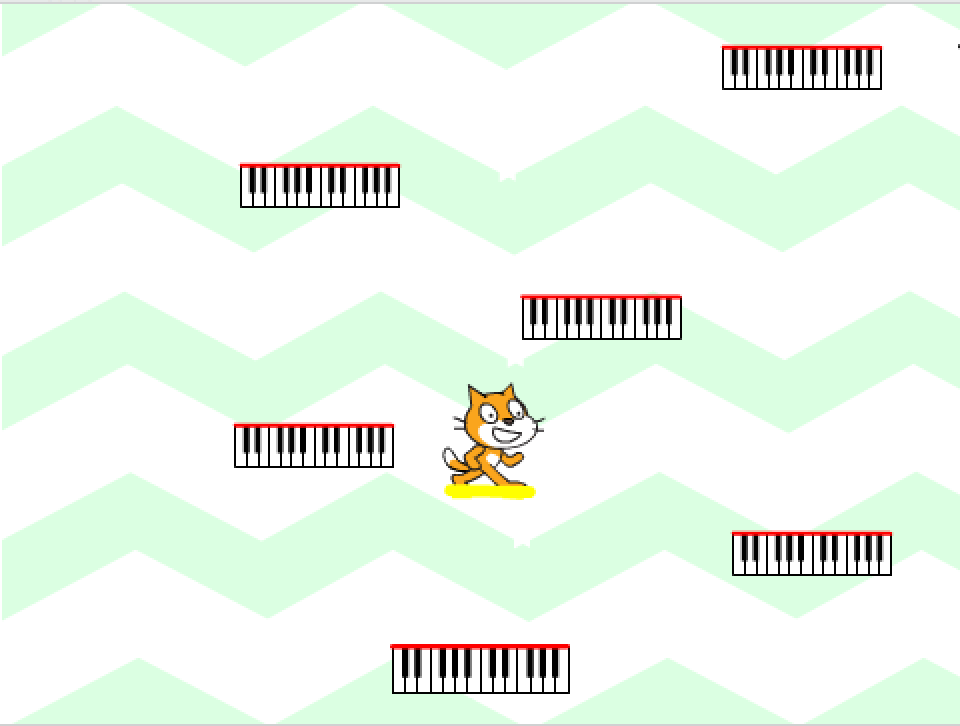
\includegraphics[width=3.5in]{preview.png}
 \end{center}
We will be building a cool game that looks like the picture above! Basically, what happens in this game is the Cat will jump up on top of the piano tiles and try to keep itself from falling to the ground. If the cat drops to the bottom, the Cat will say Game Over to signify that the player has lost. Below, there will be some directions for you to follow! If you think you can build this game without directions, don't be afraid to build it on your own!\\\\
If you have any questions about the directions or any blocks you have not used before, let me know via email or text!\\
This Project will be done on Sketch.\\
I would strongly recommend installing the \href{https://scratch.mit.edu/scratch2download/}{offline version of Scratch 2}.\\\\
\href{https://youtu.be/ZJAsPQanvtg}{Click this line to see a YouTube video of this game running!}\\
Do your best and have fun!
\begin{enumerate}
\item The Piano Tiles: Initial State (When Flag is clicked)

\begin{enumerate}[a.]
\item As soon as the game start, we want to make certain that the tiles start at the correct location. The tiles are already set up such that the cat should be able to jump from one tile to another with ease. For each tiles, set a constant for the $x$ and $y$ position. [uses: ``when flag clocked'', ``set x to'' and ``set y to'']

\item Now that the initial position of the tiles is set, we want to now let each tiles drop until it reaches the bottom of the screen. Add additional script to let the tiles steadily drop. [uses: try to figure this out on your own!]
\item Once the tiles drop to the bottom of the game screen, make sure you hide the block. [uses: ``hide'']
\item After hiding, we would want the to make more tiles the top such that the game would never end if you are a pro gamer. So, go create a clone of the piano tile. [uses: ``create clone of'']
\end{enumerate}

\item The Piano Tiles: After cloned (when I start as a clone block)
\begin{enumerate}[a.]
\item Because the tiles were hidden before cloning the piano tiles, the tile will remain hidden when we clone it from the step 1d. Make sure to show the cloned tiles right after the tile is cloned [uses: ``show''].

\item We want to start the block at the top of the screen. Set a constant for the y value for each tiles when the tile is cloned. [uses: ``set y'']

\item Now, the game would be no fun if the tiles we see are predictable. Let's make the initial x position of the cloned block be a random number between -180 and 180. [uses: try to figure this out on your own!]

\item Let the cloned block do the same thing as the original piano tile. [uses: find this out on your own!]
\end{enumerate}

\item Cat: Initial State \#1
\begin{enumerate}[a.]
\item Make sure, like the piano tiles, the cat has an appropriate initial x and y position. Tip: Position the cat above a piano tile. [uses: figure this out on your own!]
\end{enumerate}

\item Cat: Initial State \#2
\begin{enumerate}[a.]
\item We want the Cat to keep jumping forever as long as there is a tile under it. Make it such that the cat can keep jumping as long as there is a tile under the cat. Note: to make this step easier, I made the cat's feet yellow and the top of the piano tile red. [uses: figure this out on your own!]
\end{enumerate}

\item Cat: Response when Right Arrow key pressed
\begin{enumerate}[a.]
\item When we let the cat move, we want to assure that the the cat is facing the correct direction. Use a block to make sure that the cat is facing to the right when the right arrow key is pressed. [uses: figure this out on your own!]

\item When we press the right arrow button, we expect the cat to move right. So go code that up! [uses: figure this out on your own.]
\end{enumerate}

\item Cat: Response when Left Arrow key pressed
\begin{enumerate}[a.]
\item When we let the cat move, we want to assure that the the cat is facing the correct direction. Use a block to make sure that the cat is facing to the left when the left arrow key is pressed. [uses: figure this out on your own!]

\item When we press the left arrow button, we expect the cat to move left. So go code that up! [uses: figure this out on your own.]
\end{enumerate}
\newpage
\item Cat: Initial State \#3
\begin{enumerate}[a.]
\item If you saw the preview, you could see that if you go pass the screen on the left edge then you reappear on the right. Code this up! [uses: figure this out on your own!]
\end{enumerate}

\item Cat: Initial State \#4
\begin{enumerate}[a.]
\item If you saw the preview, you could see that if you go pass the screen on the right edge then you reappear on the left. Code this up! [uses: figure this out on your own!]
\end{enumerate}

\item Cat: Initial State \#5
\begin{enumerate}[a.]
\item If you saw the preview, you could see that if you go . Code this up! [uses: figure this out on your own!]
\end{enumerate}
\end{enumerate}
\end{document}
